%!TEX root = ../main.tex
\section{Kritik}
  \subsection{Unverhältnismäßige geringe Nutzung}
    \begin{frame}<beamer>{Unverhältnismäßige geringe Nutzung}
      \begin{itemize}
        \item
          Abschreckungfaktor ist nicht vorhanden.
         \item
         Umgehungsmöglichkeiten sind auch für Laien möglich.
           \begin{itemize}
         \item TOR-Netzwerk
         \item alternative Emaildienste
         \item bei SMS auf Alternativen umsteigen (zb. Whatsapp)
      \end{itemize}
        \item
       	Durch Vorratsdatenspeicherung hätte weder 9/11 als auch die Attentate in Großbritannien 2005 verhindert werden können
      \end{itemize}
    \end{frame}

\begin{frame}<beamer>{Schwere Strafdaten in Deutschland Statstik}
\begin{itemize}
        \item Schwere Strafdaten in Deutschland Statstik
        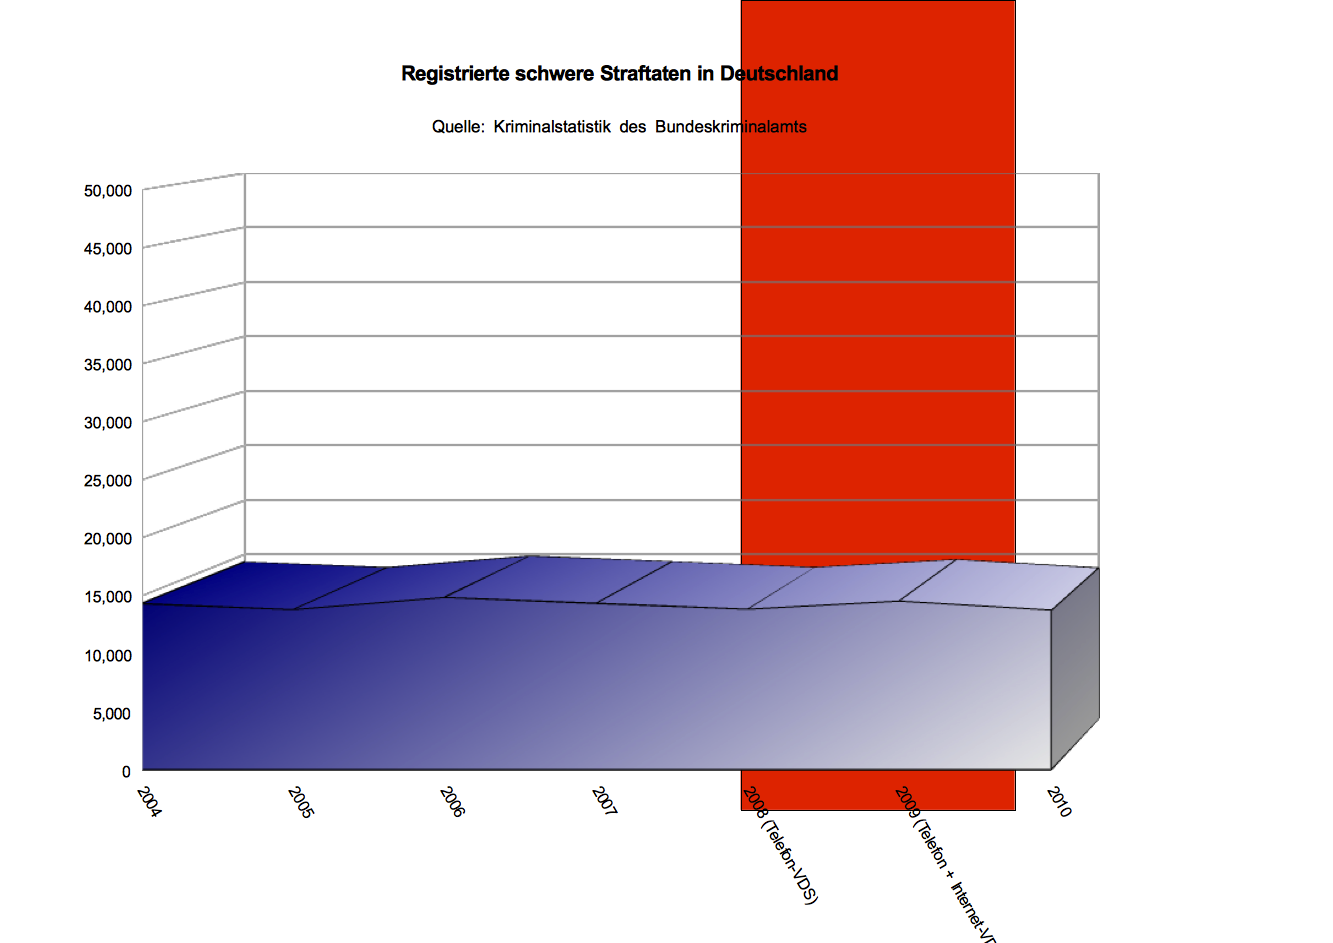
\includegraphics[height=1\textheight]{sections/img/schwere_verbrechen_in_DE.png}
    \end{itemize}
    \end{frame}
    
    \begin{frame}<beamer>{Schwere Verbrechen in Deutschland Aufklärung Statistik}
\begin{itemize}
        \item Schwere Verbrechen in Deutschland Aufklärung Statistik
        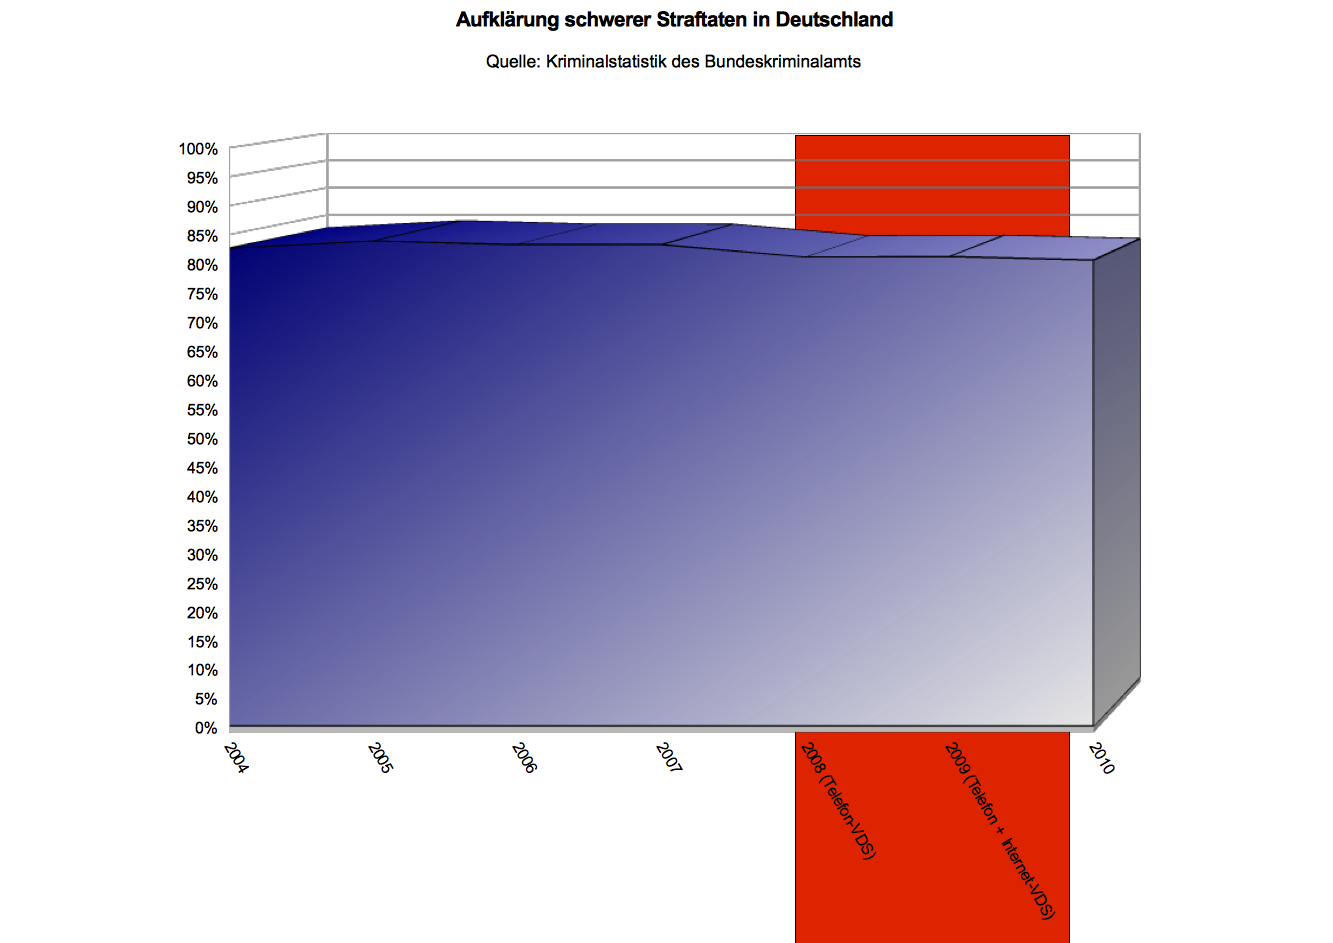
\includegraphics[height=1\textheight]{sections/img/aufklaerung_in_DE.png}
    \end{itemize}
    \end{frame}
      \begin{frame}<beamer>{Internetstrafdaten in Deutschland Statistik}
\begin{itemize}
        \item Internetstrafdaten in Deutschland Statistik
        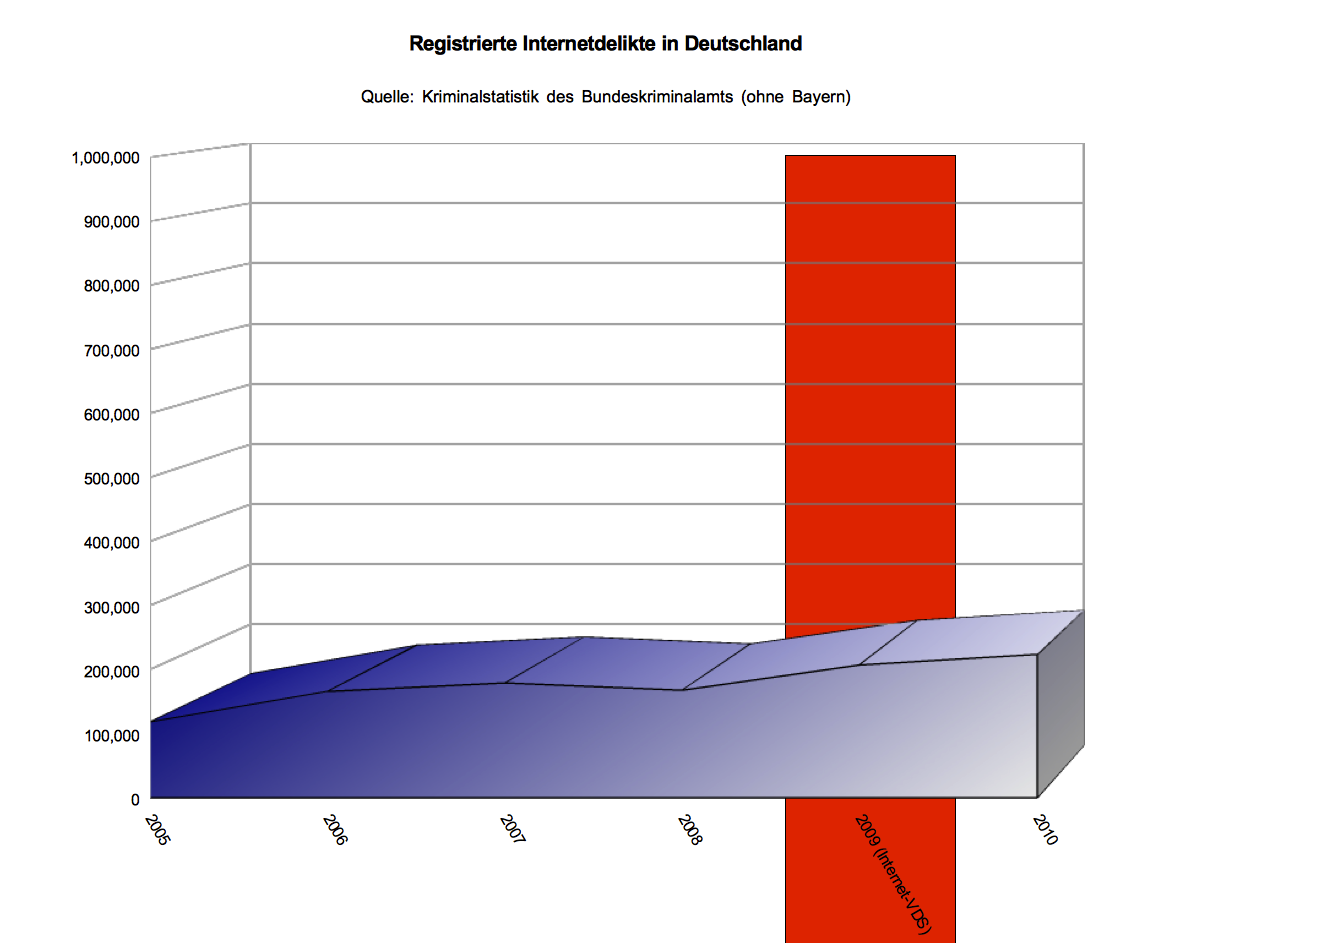
\includegraphics[height=1\textheight]{sections/img/internet_delikte_in_DE.png}
    \end{itemize}
    \end{frame}
          \begin{frame}<beamer>{Internetstrafdaten in Deutschland Aufklärung Statistik}
\begin{itemize}
        \item Internetstrafdaten in Deutschland Aufklärung Statistik
        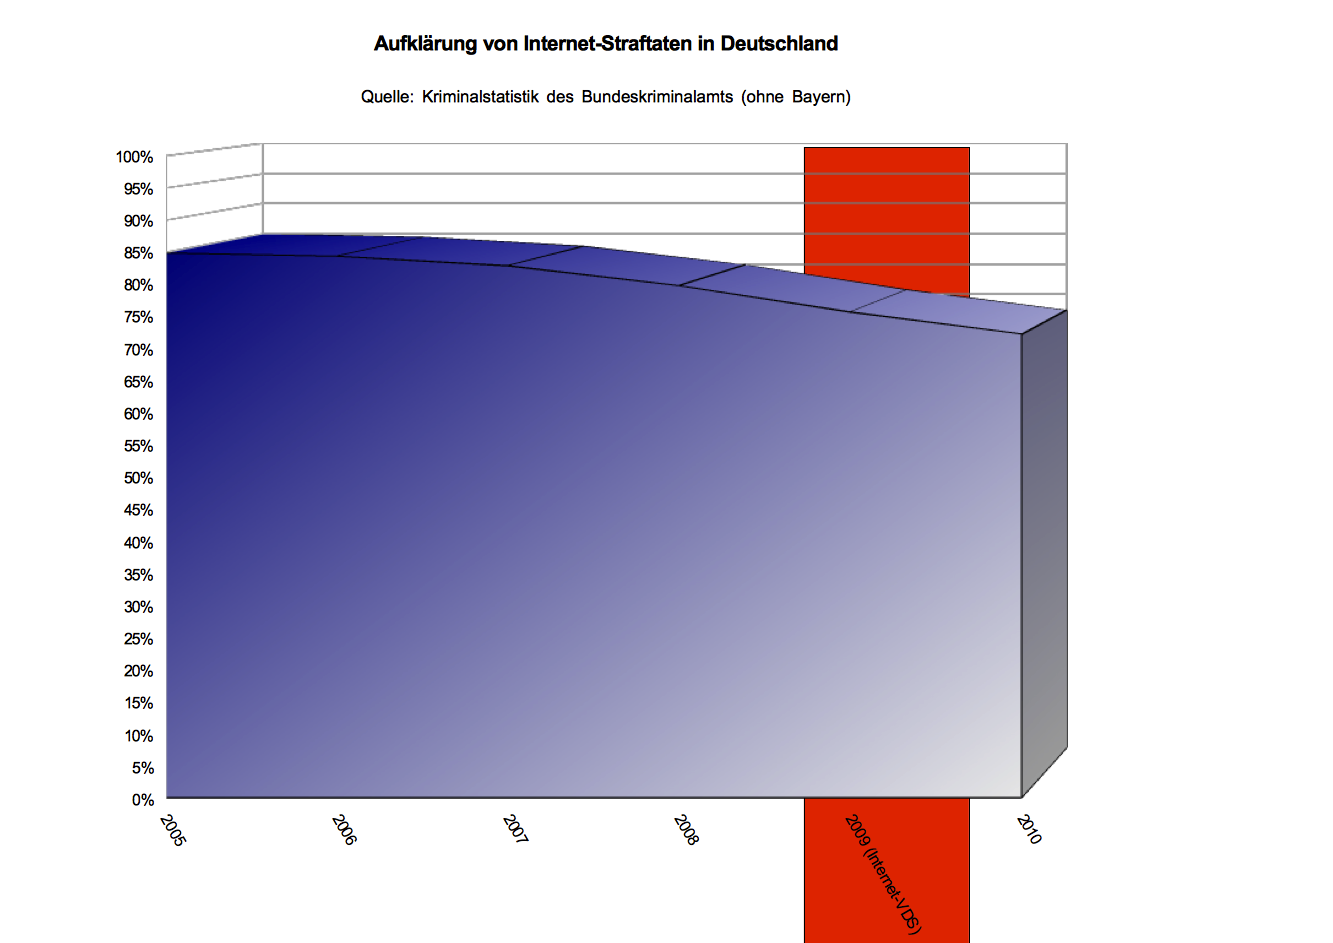
\includegraphics[height=1\textheight]{sections/img/aufklaerung_internetdelikte_DE.png}
    \end{itemize}
    \end{frame}
              \begin{frame}<beamer>{Aufklärungsquote Allgmein}
\begin{itemize}
        \item Aufklärungsquote Allgmein
        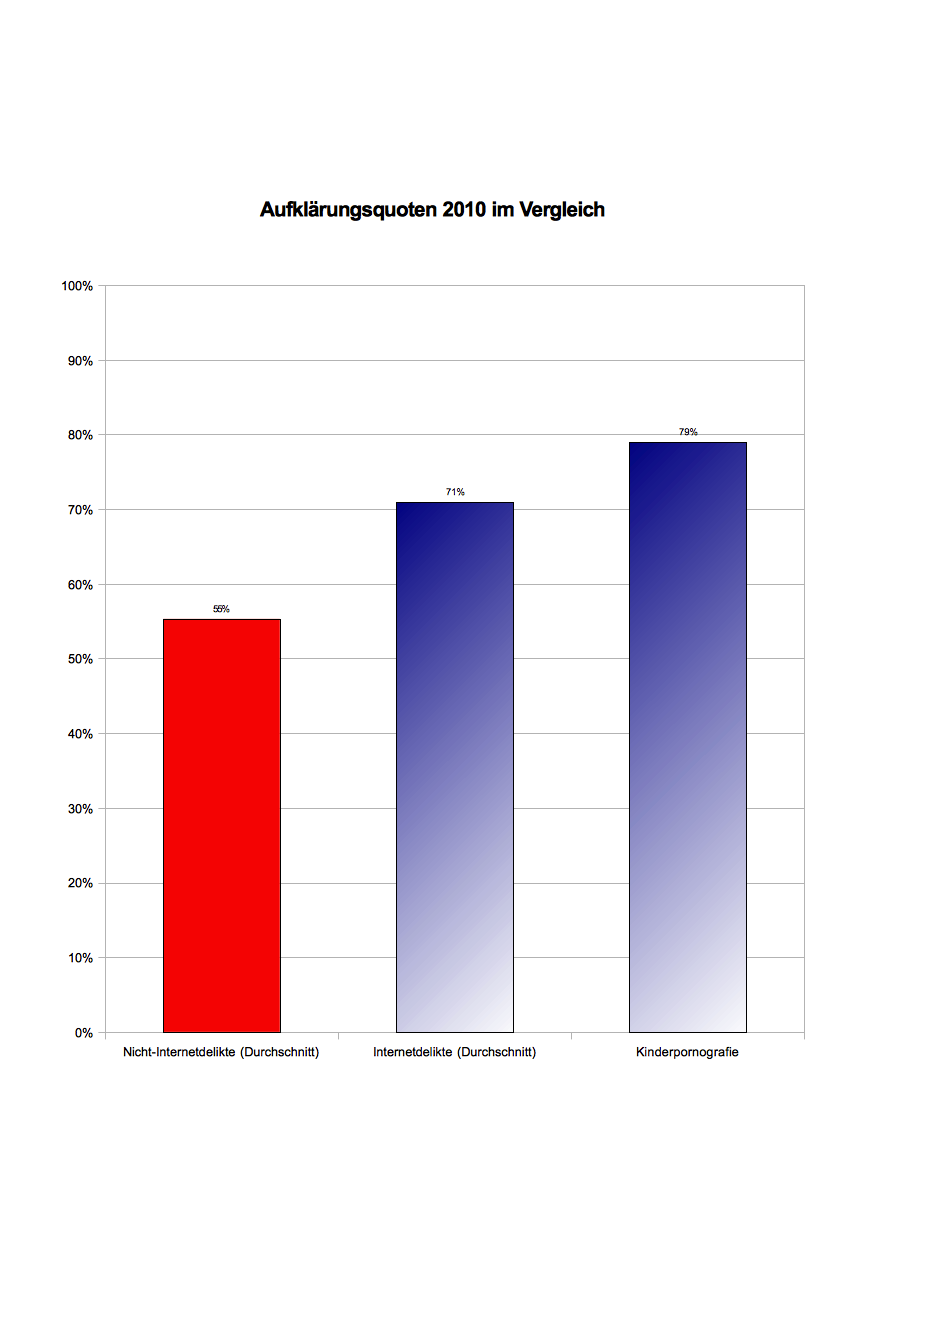
\includegraphics[height=1\textheight]{sections/img/aufklaerung.png}
    \end{itemize}
    \end{frame}
              \begin{frame}<beamer>{Interpretation der Statistik des Bundeskriminalamtes}
\begin{itemize}
        \item Die VDS brachte keine Erhöhte Aufklärungsquote
        \item Es konnte keine Senkung der Kriminalitätsrate festgestellt werden
        \item Die Aufklärungsrate der Internetstraftaten sank im Zeitraum der VDS
    \end{itemize}
    \end{frame}



  \subsection{Missbrauch und Irrtumsrisiko}
    \begin{frame}<beamer>{Missbrauch und Irrtumsrisiko}
      \begin{itemize}
        \item
          Telekommunikationsdaten haben eine sehr hohe Aussagekraft
      \begin{itemize}
         \item mit Methoden von Data-mining können scheinbar belanglose Daten eine hohe Aussagekraft bekommen
      \end{itemize}
        \item
          Rückschlüsse auf die gesamte Lebensituation möglich
 \item viele Interessensgruppen haben Interesse an den sensiblen Daten
          \begin{itemize}
         \item Behörden/Staat
         \item politische Gruppierungen
         \item Personen aus Privatenumfeld
      \end{itemize}
 
      \end{itemize}
    \end{frame}

  \subsection{Juristische Argumente}
    \begin{frame}<beamer>{Juristische Argumente}
      \begin{itemize}
        \item Verstoß gegen Europarecht
           \begin{itemize}
         \item Verstoß gegen Gemeinschaftsgrundrechte
      \end{itemize}
        \item Verstoß gegen deutsches Recht
        \item Verstoß gegen die Europäische Menschenrechtskonvention
      \end{itemize}
    \end{frame}

  \subsection{Zukunft informelle Selbstbestimmung}
    \begin{frame}<beamer>{Zukunft informelle Selbstbestimmung}
      \begin{itemize}
        \item
          todo
  

      \end{itemize}
    \end{frame}

  \subsection{Demonstrationen}
    \begin{frame}<beamer>{Demonstrationen}
      \begin{itemize}
        \item
          todo
  
      \end{itemize}
    \end{frame}
